\documentclass{standalone}
\usepackage{tikz}
\usepackage{ctex,siunitx}
\usepackage{tkz-euclide}
\usepackage{amsmath}
\usetikzlibrary{patterns, calc}
\usetikzlibrary {decorations.pathmorphing, decorations.pathreplacing, decorations.shapes,}
\begin{document}
\small
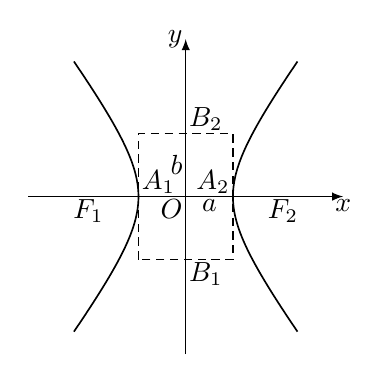
\begin{tikzpicture}[>=latex,scale=1,inner sep=1pt]
  \draw[thin,->](-2,0)--(2,0)node[below]{$x$};
  \draw[thin,->](0,-2.0)--(0,2.0)node[left]{$y$};
  \tkzDefPoints{0/0/O,-1/0/F1,1/0/F2}
  \draw[semithick,domain=-65:65,samples=200] plot ({0.6/cos(\x)},{0.8*tan(\x)});
  \draw[semithick,domain=-65:65,samples=200] plot ({-0.6/cos(\x)},{0.8*tan(\x)});
  \draw[densely dashed](-0.6,-0.8)rectangle(0.6,0.8);
  \tkzLabelPoint[below left](F1){$F_1$}
  \tkzLabelPoint[below right](F2){$F_2$}
  \tkzLabelPoints[below left](O)
  \node at (0,0.8)[above right]{$B_2$};
  \node at (0,-0.8)[below right]{$B_1$};
  \node at (-0.6,0)[above right]{$A_1$};
  \node at (0.6,0)[above left]{$A_2$};
  \node at (0.3,0)[below]{$a$};
  \node at (0,0.4)[left]{$b$};
\end{tikzpicture}
\end{document}